\documentclass[./main_en.tex]{subfiles}
\graphicspath{{\subfix{./figs}}}

% ------------ main document ------------
\begin{document}
\nolinenumbers

% style setup
\newpage
\renewcommand{\headrulewidth}{0pt}
\thispagestyle{fancy}
%... then configure it
\fancyhf{} % Clear all header and footer fields.
\fancyfoot{} % clear all footer fields
\fancyfoot[C]{\thepage}

\par \hfill
\vspace{40mm}
\begin{adjustwidth}{45pt}{45pt}
\begin{center}
    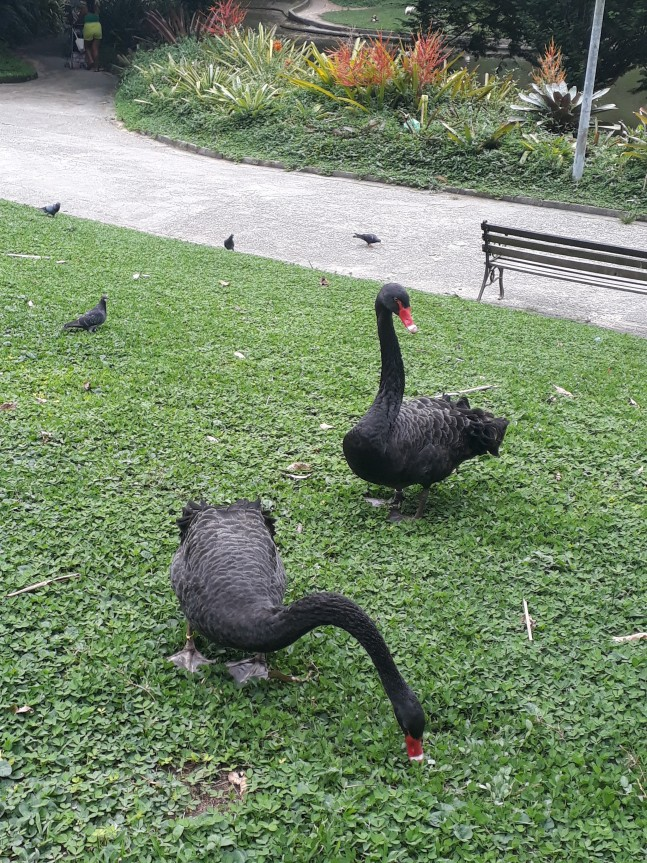
\includegraphics[scale=1]{fig_swan.jpg}\\
\end{center}
\vspace{10mm}
\noindent \textsf{On February 16, 2023, at 3:23 PM, two black swans were observed in the park behind the Palácio das Laranjeiras, Rio de Janeiro, Brazil. A single black swan would already be sufficient to prove that \textit{not all swans are white}.}
\end{adjustwidth}
\clearpage
\end{document}